\section{实验结果与分析}\label{sec:experiment}

\subsection{实验环境与设置}

本章使用 LEVIR-Ship 数据集上的实验记录，对 DRENet、FCOS 和 YOLO26 进行比较。指标部分保留 AP50、AP50-95、Precision、Recall 与 F1；工程侧另记录 FPS、参数量和 FLOPs。训练配置、权重文件、运行日志和结果文档均已保存，后续表格和图示可追溯到对应产物。

除离线训练和测试外，系统侧推理流程也完成联调，相关输出可用于第五章的任务管理与结果回看说明。

\subsection{三模型主对比结果}

三模型核心结果见表~\ref{tab:ch4_baselines}，对应日志和权重均已留存。

\begin{table}[htbp]
  \centering
  \caption{三模型在 LEVIR-Ship 数据集上的主对比结果}
  \label{tab:ch4_baselines}
  \begin{tabular}{lccccc}
    \toprule
    模型 & AP50 & AP50-95 & Precision & Recall & F1 \\
    \midrule
    DRENet & 0.7949 & 0.2919 & 0.4927 & 0.8511 & 0.6241 \\
    FCOS & 0.7700 & 0.2850 & -- & 0.4050 & -- \\
    YOLO26 & 0.7950 & 0.3170 & 0.8430 & 0.7220 & 0.7778 \\
    \bottomrule
  \end{tabular}
\end{table}

\begin{figure}[H]
  \centering
  
\includegraphics[width=0.96\textwidth]{img/ch4_main_comparison_chart.png}
  \caption{三模型主对比结果的指标可视化}
  \label{fig:ch4_main_comparison_chart}
\end{figure}

表~\ref{tab:ch4_baselines} 与图~\ref{fig:ch4_main_comparison_chart} 中，YOLO26 和 DRENet 的 AP50 几乎相同，分别为 0.7950 和 0.7949，FCOS 为 0.7700。仅从 AP50 看，专项方法和成熟 one-stage 路线在该数据集上都能完成基本检出，二者差距并不体现在这一项主指标上。

差异主要出现在 AP50-95、Precision 和 Recall 上。YOLO26 的 AP50-95 为 0.3170，高于 DRENet 的 0.2919 和 FCOS 的 0.2850，说明在更严格的 IoU 阈值下，它的边框位置更稳。DRENet 的 Recall 为 0.8511，高于 YOLO26 的 0.7220，但 Precision 只有 0.4927，低于 YOLO26 的 0.8430。也就是说，DRENet 更愿意保留可疑目标，代价是误检更多；YOLO26 对候选框筛选更严格，输出更干净。

FCOS 的 AP50 和 AP50-95 均低于前两者。在当前实验条件下，通用 anchor-free 基线没有表现出优势。不过 FCOS 仍有保留意义：它给后文讨论专项设计和 one-stage 部署路线时提供了另一条参照线。

\subsection{效率与部署属性分析}

除精度指标外，工程部署场景还要关注模型在速度和复杂度方面的表现。当前可用效率结果如表~\ref{tab:ch4_efficiency} 所示。

\begin{table}[htbp]
  \centering
  \caption{三模型效率与复杂度对比}
  \label{tab:ch4_efficiency}
  \small
  \begin{tabular}{lccc}
    \toprule
    模型 & FPS & Params(M) & FLOPs(G) \\
    \midrule
    DRENet & 121.8993 & 4.7882 & 4.2057 \\
    FCOS & 45.9559 & 32.1664 & 123.0 \\
    YOLO26 & 69.0625 & 2.5042 & 3.6939 \\
    \bottomrule
  \end{tabular}
\end{table}

效率表中的趋势和精度表并不完全相同。DRENet 在当前记录中 FPS 最高，说明其推理速度较突出。YOLO26 的参数量为 2.5042M、FLOPs 为 3.6939G，模型规模更小。FCOS 的参数量和计算量较高，整体效率低于前两者。三模型效率与复杂度对比的可视化见图~\ref{fig:ch4_efficiency_chart}。

\begin{figure}[H]
  \centering
  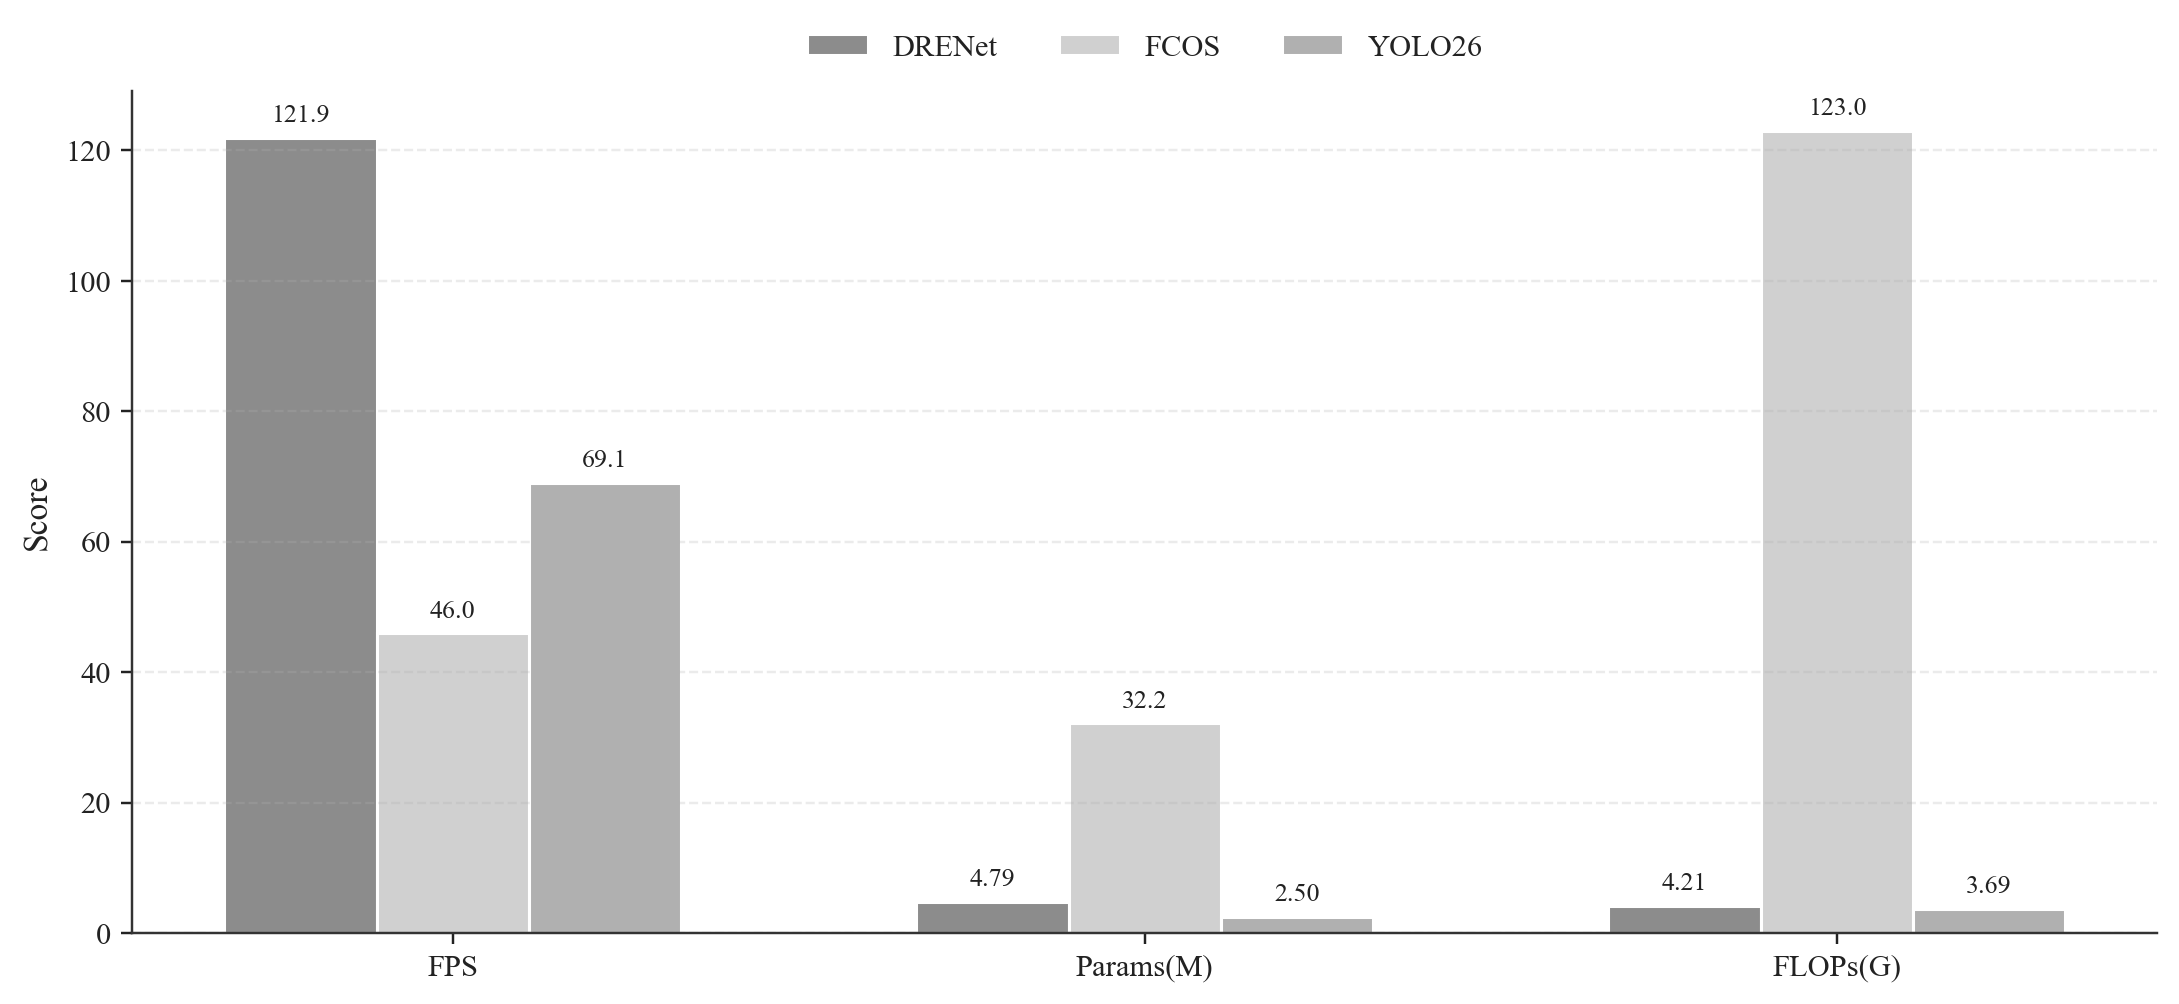
\includegraphics[width=0.92\textwidth]{img/ch4_efficiency_chart.png}
  \caption{三模型效率与复杂度对比柱状图}
  \label{fig:ch4_efficiency_chart}
\end{figure}

把精度和效率放在一起读，DRENet 在召回和速度方面优势明显，YOLO26 在定位质量、误检控制和模型规模之间更均衡，FCOS 则提供 anchor-free 路线的对照。为综合展示三模型在精度与效率各维度上的表现，本文绘制了多维度雷达图（见图~\ref{fig:ch4_radar_chart}），其中参数效率和计算效率取逆指标（越小越优）进行归一化。

\begin{figure}[H]
  \centering
  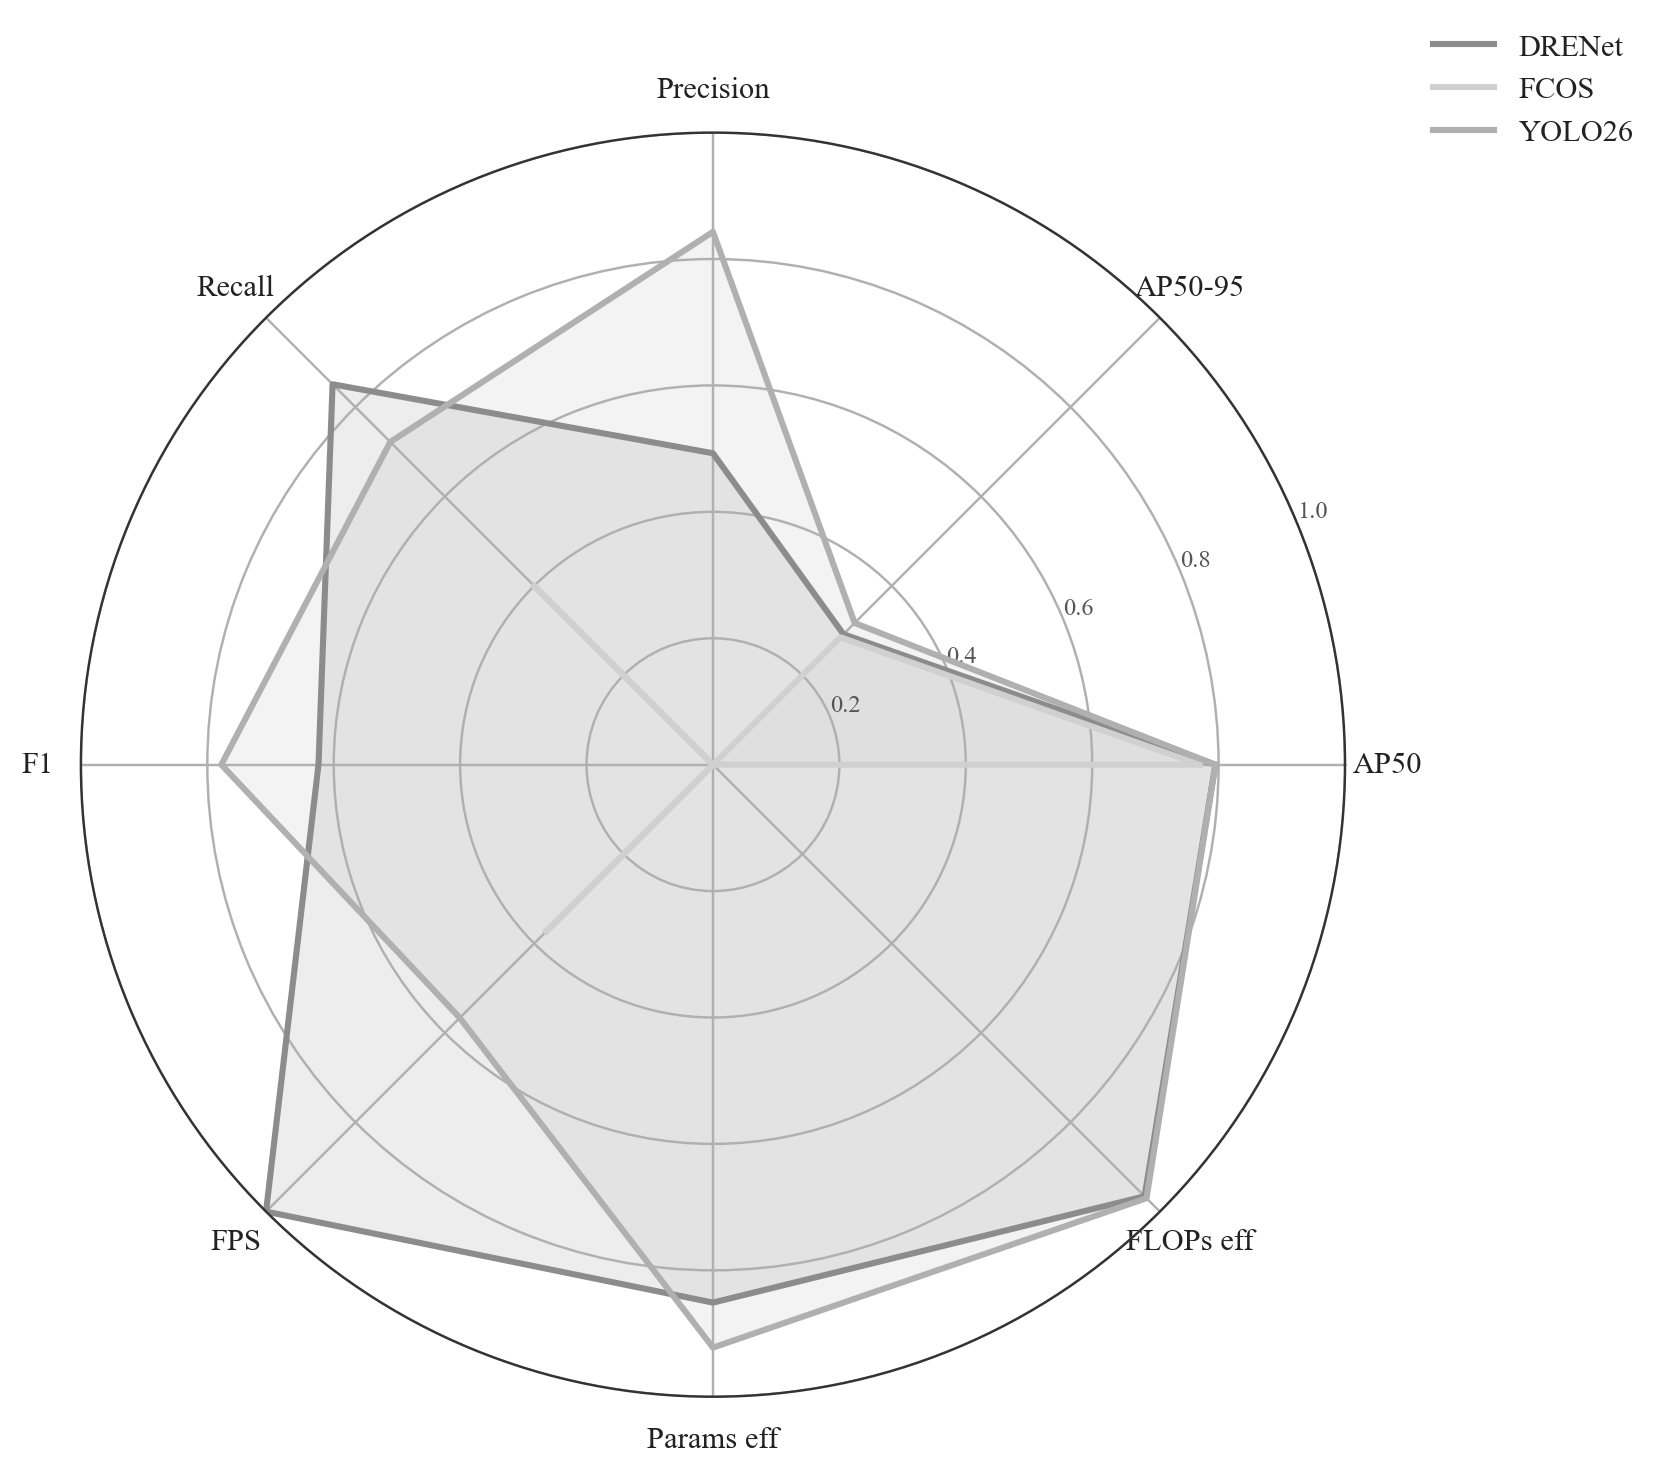
\includegraphics[width=0.65\textwidth]{img/ch4_radar_chart.png}
  \caption{三模型多维度综合雷达图}
  \label{fig:ch4_radar_chart}
\end{figure}

\subsection{模型逐项分析}

\subsubsection{DRENet 结果分析}

DRENet 在本文结果中最醒目的特点是 Recall 高。当前正式结果中，它的 Recall 为 0.8511，高于 YOLO26，说明该模型在复杂背景和弱纹理目标上更倾向于保留候选框。若任务目标是先尽可能发现可疑船舶，再由后续流程复核，这种取向有实际价值。

DRENet 的问题也很直接：Precision 为 0.4927，误检压力较大。近岸区域、港区设施和背景边缘纹理都可能被它保留下来。因此，DRENet 更适合作为召回优先的候选方案；若要进入更严格的部署流程，还需要通过阈值、后处理或融合策略继续压低误检。

\subsubsection{FCOS 结果分析}

FCOS 的 AP50 为 0.7700，低于 DRENet 与 YOLO26。在当前中分辨率遥感微小船舶任务中，通用 anchor-free 路线没有占到优势。不过 FCOS 的结构清晰、范式明确，保留这组结果后，专项设计和 one-stage 路线在该任务中的差异更容易讨论。

\subsubsection{YOLO26 结果分析}

YOLO26 的 AP50 与 DRENet 基本持平，但 AP50-95、Precision 和 F1 更高。Precision 达到 0.8430，说明在当前阈值设置下，它对复杂背景中的伪目标压制更强，输出框更少出现大面积冗余。

工程侧也更偏向 YOLO26。它的训练链路较成熟，接口封装也相对直接，因此在系统接入时适配成本较低。与 DRENet 配合时，它也可以在误检控制上形成互补。

\subsection{定性样例与误差分析}

定量指标只能给出整体趋势，定性样例可以进一步呈现不同错误类型。本文整理成功检测、漏检和误检样例，并结合表~\ref{tab:ch4_baselines} 的指标解释模型行为。

\subsubsection{成功检测样例}

成功样例中，DRENet 在海面纹理较弱、目标尺寸较小的图像上仍能给出响应，这与它召回偏高的定量结果相符。YOLO26 的结果更整洁，尤其在多目标和常规场景中，预测框与标注框的匹配更稳定。FCOS 也能在部分样例中完成定位，但波动更大。如图~\ref{fig:ch4_success_cases} 所示，各模型在代表样本上的检测风格存在明显差异。

\begin{figure}[H]
  \centering
  
\includegraphics[width=0.95\textwidth]{img/ch4_success_cases.png}
  \caption{三模型成功检测样例对比}
  \label{fig:ch4_success_cases}
\end{figure}

\subsubsection{漏检样例}

漏检样例中，三类模型都会遗漏目标，但遗漏位置和原因不完全相同。如图~\ref{fig:ch4_miss_cases} 所示，标注框与预测框之间的缺失主要出现在弱纹理、小尺寸以及背景对比度不足的区域。

\begin{figure}[H]
  \centering
  
\includegraphics[width=0.95\textwidth]{img/ch4_miss_cases.png}
  \caption{三模型漏检样例对比}
  \label{fig:ch4_miss_cases}
\end{figure}

\subsubsection{误检样例}

误检样例则更能解释 Precision 差异。DRENet 更容易把复杂背景纹理保留下来；YOLO26 偶尔会在边缘背景区域产生额外响应；FCOS 也存在误检，但数量和位置与前两者不同。如图~\ref{fig:ch4_false_positive_cases} 所示，三者误检分布位置并不一致。

\begin{figure}[H]
  \centering
  
\includegraphics[width=0.95\textwidth]{img/ch4_false_positive_cases.png}
  \caption{三模型误检样例对比}
  \label{fig:ch4_false_positive_cases}
\end{figure}

把这些样例和表~\ref{tab:ch4_baselines} 对照后可以发现，DRENet 与 YOLO26 的差别并不是单纯分数高低。DRENet 更偏向“先检出”，复杂背景下误检会变多；YOLO26 更偏向输出稳定和边框质量，弱目标场景下可能漏掉一部分目标。FCOS 则继续作为 anchor-free 路线的补充参照。

\subsection{消融实验}

为了说明主表中 Precision 与 Recall 的差异，实验部分补充置信度阈值和输入尺寸两组消融。前者观察候选框筛选松紧变化后各模型的响应，后者观察推理输入尺寸变化对检测结果的影响。

\subsubsection{阈值消融分析}

阈值消融固定 IoU 阈值为 0.50，置信度阈值取 0.15、0.25 和 0.35。本文主要观察阈值升高后 Precision、Recall 和 F1 的变化情况。三模型结果见表~\ref{tab:ch4_threshold_ablation}。

\begin{table}[htbp]
  \centering
  \small
  \caption{三模型阈值消融结果}
  \label{tab:ch4_threshold_ablation}
  \begin{tabular}{@{}llccccp{4.2cm}@{}}
    \toprule
    模型 & 设置 & AP50 & Precision & Recall & F1 & 结论 \\
    \midrule
    DRENet & conf=0.15 & 0.6616 & 0.6441 & 0.7935 & 0.7110 & 低阈值召回更高，但误检增加 \\
    DRENet & conf=0.25 & 0.6616 & 0.7331 & 0.7663 & 0.7493 & 默认值更均衡 \\
    DRENet & conf=0.35 & 0.6616 & 0.7778 & 0.7355 & 0.7561 & 精度继续上升，召回下降 \\
    FCOS & conf=0.15 & 0.7389 & 0.7283 & 0.8351 & 0.7781 & 低阈值检出更充分 \\
    FCOS & conf=0.25 & 0.7389 & 0.7621 & 0.8297 & 0.7944 & 默认值已较均衡 \\
    FCOS & conf=0.35 & 0.7389 & 0.7761 & 0.8225 & 0.7986 & F1 略优于 0.25 \\
    YOLO26 & conf=0.15 & 0.6661 & 0.6412 & 0.7899 & 0.7078 & 召回提升明显，但误检偏多 \\
    YOLO26 & conf=0.25 & 0.6661 & 0.7527 & 0.7609 & 0.7568 & 综合表现最均衡 \\
    YOLO26 & conf=0.35 & 0.5914 & 0.8248 & 0.6993 & 0.7569 & 精度最高，但 AP50 与召回下降 \\
    \bottomrule
  \end{tabular}
\end{table}

\begin{figure}[H]
  \centering
  
\includegraphics[width=0.98\textwidth]{img/ch4_threshold_trend.png}
  \caption{三模型阈值消融趋势图}
  \label{fig:ch4_threshold_trend}
\end{figure}

表~\ref{tab:ch4_threshold_ablation} 和图~\ref{fig:ch4_threshold_trend} 显示，阈值升高后，三模型的 Precision 大多上升，Recall 大多下降。这一趋势符合候选框筛选逻辑，也说明后处理阈值会明显改变遥感微小船舶检测结果。

DRENet 对阈值较敏感。低阈值会进一步放大它的召回倾向，但误检也随之增加；阈值提高到 0.35 后，Precision 升至 0.7778，Recall 降至 0.7355。若系统需要在检出率和误检数量之间取一个中间位置，0.25 比 0.15 和 0.35 更适合作为默认值。

FCOS 和 YOLO26 的变化则更细。FCOS 在当前稳定权重下，阈值由 0.25 提高到 0.35 时，F1 从 0.7944 小幅升至 0.7986，说明这组权重下略高阈值能压掉一部分冗余候选。YOLO26 在 0.25 时 AP50、Precision 和 Recall 的组合更均衡；继续升到 0.35 后，Precision 到 0.8248，但 AP50 与 Recall 同时下降。综合 AP50、Precision、Recall 和 F1，0.25 可作为后续实验和系统推理的主要阈值设置。

\subsubsection{输入尺寸敏感性分析}

输入尺寸敏感性分析固定置信度阈值为 0.25、IoU 阈值为 0.50，只改变推理阶段的输入尺寸。由于 FCOS 的推理接口不支持本节设置的输入尺寸调整，本节主要分析 YOLO26 的变化，结果见表~\ref{tab:ch4_size_ablation}。

\begin{table}[htbp]
  \centering
  \small
  \caption{YOLO26 输入尺寸敏感性分析结果}
  \label{tab:ch4_size_ablation}
  \begin{tabular}{lccccc}
    \toprule
    设置 & AP50 & Precision & Recall & F1 & 结论 \\
    \midrule
    imgsz=512 & 0.6661 & 0.7527 & 0.7609 & 0.7568 & 基线稳定 \\
    imgsz=640 & 0.6737 & 0.7543 & 0.7953 & 0.7743 & 综合表现最优 \\
    imgsz=800 & 0.6564 & 0.6827 & 0.7989 & 0.7362 & 召回提高但误检增加 \\
    \bottomrule
  \end{tabular}
\end{table}

\begin{figure}[H]
  \centering
  
\includegraphics[width=0.86\textwidth]{img/ch4_size_trend.png}
  \caption{输入尺寸敏感性趋势图}
  \label{fig:ch4_size_trend}
\end{figure}

表~\ref{tab:ch4_size_ablation} 与图~\ref{fig:ch4_size_trend} 显示，YOLO26 在 640 输入下取得本组最高 AP50 和 F1，Precision 与 Recall 也保持较好平衡。当输入尺寸继续增至 800 时，Recall 略有提高，但 Precision 和 F1 明显下降，说明更大的推理输入会带来更多候选目标，同时也更容易引入误检。
